% AcademiX - Informe Entrega 1
% Compilar con pdfLaTeX (Overleaf: Menu > Compiler > pdfLaTeX).
% Fuente: docs/deliveries/0/*.md (scope, requirements, user-stories, architecture,
% architecture-diagram, roadmap, glossary, discovery-notes, checklist) y mockups/.
\documentclass[letterpaper,10pt]{article}

\usepackage[left=1.15cm,right=1.15cm,top=1.05cm,bottom=1.05cm]{geometry}
\usepackage[utf8]{inputenc}
\usepackage[T1]{fontenc}
\usepackage[spanish,es-noshorthands]{babel}
\usepackage{helvet}
\usepackage{xcolor}
\usepackage{enumitem}
\usepackage{microtype}
\usepackage{graphicx}
\usepackage{tabularx}
\usepackage{longtable}
\usepackage{array}
\usepackage{multicol}
\usepackage{tikz}
\usepackage{hyperref}

\usetikzlibrary{arrows.meta,positioning}

\definecolor{navy}{HTML}{1E3A5F}
\definecolor{amber}{HTML}{A16207}
\definecolor{line}{HTML}{CBD5E1}
\definecolor{soft}{HTML}{F8FAFC}
\definecolor{slate}{HTML}{64748B}

\renewcommand{\familydefault}{\sfdefault}
\pagestyle{empty}
\setcounter{secnumdepth}{0}
\setlength{\parindent}{0pt}
\setlength{\parskip}{3pt}
\setlist[itemize]{leftmargin=*,topsep=1pt,itemsep=1pt,parsep=0pt}
\setlist[enumerate]{leftmargin=*,topsep=1pt,itemsep=1pt,parsep=0pt}
\hypersetup{colorlinks=true,urlcolor=navy,linkcolor=navy}

\emergencystretch=2em
\newcolumntype{Y}{>{\raggedright\arraybackslash}X}
\newcommand{\tightcaption}[1]{{\footnotesize\textbf{#1}}}
\newcommand{\st}[1]{\textcolor{amber}{\textbf{#1}}}
\renewcommand{\arraystretch}{1.05}

\begin{document}

\begin{center}
{\LARGE\bfseries\color{navy} AcademiX: LMS multi-tenant universitario}\\
{\large Entrega 1}\\
IIC3143 Desarrollo de Software · Equipo AcademiX · \today
\end{center}

\section{1. Razón y justificación de la solución}

\textbf{Introducción y contexto.} Las universidades usan plataformas LMS para centralizar cursos, material académico, evaluaciones, entregas y comunicación. En la práctica, buena parte del flujo académico termina repartida entre el LMS institucional, planillas de cálculo, correos, calendarios externos y carpetas de archivos. La consecuencia es una experiencia fragmentada para los tres actores que sostienen un curso semestral: estudiantes, cuerpo docente y administración académica.

\textbf{Problema y motivación.} El problema no es la falta de funcionalidades en los LMS existentes, sino la baja integración del flujo crítico de un curso: \emph{curso $\rightarrow$ módulos $\rightarrow$ material $\rightarrow$ evaluaciones $\rightarrow$ entregas $\rightarrow$ corrección $\rightarrow$ publicación de notas $\rightarrow$ libro de notas}. Se observan cuatro síntomas: (i) el estudiante no distingue con rapidez qué estudiar, qué entregar y qué notas ya fueron publicadas; (ii) las notas y ponderaciones se gestionan fuera de la plataforma; (iii) el material queda como archivo pasivo, sin vínculo con la evaluación que lo usa; y (iv) las instituciones necesitan aislar datos y escalar por universidad. Este diagnóstico surge principalmente de la experiencia del equipo utilizando Canvas. En esta etapa no se realizaron entrevistas ni mediciones formales, por lo que se trata de una observación inicial y se reconoce esa limitación. La propuesta busca, por tanto, que las tareas principales de un curso puedan realizarse de forma continua dentro de una misma plataforma, reduciendo la dependencia de planillas, carpetas, calendarios y otras herramientas externas.

\textbf{Valor de negocio.} Para la institución, el valor está en reducir la dependencia de planillas externas, dejar evidencia y trazabilidad de entregas y calificaciones, mantener control sobre los datos de cada universidad y operar varias instituciones sin mezclar información. Para el cuerpo docente, en configurar y calcular calificaciones dentro de la plataforma y controlar cuándo se publican. Para el estudiante, en claridad sobre sus calificaciones y su avance en el curso. Se busca una integración del flujo académico crítico, más que un posicionarse en paridad funcional con plataformas como Canvas o Moodle.

\section{2. Interesados y usuarios}

\textbf{Resumen de interesados} (afectados por el resultado, no necesariamente usuarios diarios):

{\small
\begin{tabularx}{\textwidth}{|p{3.15cm}|Y|Y|}
\hline
\textbf{Interesado} & \textbf{Interés principal} & \textbf{Qué espera de AcademiX} \\
\hline
Universidad / Dirección de docencia & Continuidad operacional, seguridad y control institucional de los datos. & Operar sus cursos sin fuga de información entre instituciones. \\
\hline
Departamento académico & Administrar periodos, cursos, secciones y equipos docentes. & Coordinar la oferta académica y los permisos del semestre. \\
\hline
Cuerpo docente & Organizar material, evaluaciones, corrección y calificaciones. & Un único lugar para el ciclo completo del curso. \\
\hline
Equipo técnico del proyecto & Arquitectura mantenible, desplegable y observable en un semestre. & Un alcance acotado que se pueda construir y demostrar. \\
\hline
\end{tabularx}}

\textbf{Resumen de usuarios} (roles que operan el sistema; un usuario puede tener distintos roles según tenant y curso):

{\small
\begin{tabularx}{\textwidth}{|p{3.15cm}|Y|Y|}
\hline
\textbf{Usuario} & \textbf{Rol funcional} & \textbf{Acciones clave} \\
\hline
Administrador de tenant & Gestión institucional dentro de una universidad. & Usuarios, periodos académicos, cursos, secciones e inscripciones. \\
\hline
Docente & Dueño del curso. & Configura curso, módulos, material, evaluaciones y ponderaciones; corrige y libera notas. \\
\hline
Ayudante docente & Apoyo delegado con permisos acotados. & Corrección, comentarios, material, anuncios y recorrecciones según permiso. \\
\hline
Estudiante & Consumidor del flujo académico. & Revisa cursos y pendientes, identifica a su cuerpo docente, consume material, entrega y consulta notas liberadas. \\
\hline
\end{tabularx}}

\section{3. Necesidades a resolver}

\textbf{Descripción del producto.} AcademiX es un LMS multi-tenant para instituciones de educación superior. Cada universidad opera como un tenant aislado, con sus propios usuarios, cursos, archivos, evaluaciones y notas. El producto organiza el semestre alrededor del curso: el material vive en módulos publicables u ocultables, las evaluaciones tienen fecha, puntaje y ponderación, las entregas dejan evidencia con estado, la corrección admite nota y comentarios, el sistema calcula el promedio según las ponderaciones configuradas y la publicación de notas es una acción explícita del docente.

{\small
\begin{tabularx}{\textwidth}{|p{3.05cm}|Y|Y|}
\hline
\textbf{Necesidad} & \textbf{Rasgo del producto} & \textbf{Beneficio} \\
\hline
Saber qué hacer ahora & Dashboard con cursos, evaluaciones próximas y anuncios recientes. & Menos plazos perdidos y menos búsqueda manual. \\
\hline
Saber quién responde por el curso & Cuerpo docente de la sección visible con nombre y rol. & El estudiante sabe a quién dirigirse, sin exponer participantes ajenos al curso. \\
\hline
Centralizar el material & Módulos con estado publicado u oculto, archivos y enlaces. & Material vinculado al curso y visible sólo cuando el docente lo decide. \\
\hline
Gestionar evaluaciones & Evaluaciones con fecha, puntaje y ponderación; entregas con estado. & Evidencia del envío y control del ciclo completo. \\
\hline
Calificar con transparencia & Cálculo de promedios según ponderaciones, liberación manual y libro de notas. & El docente deja de depender de planillas; el estudiante ve sólo lo liberado y sabe si su promedio es parcial. \\
\hline
Aislar instituciones & Resolución de tenant por request, base de datos por tenant y roles contextuales. & Menor riesgo de acceso cruzado y escalamiento por universidad. \\
\hline
\end{tabularx}}

\textbf{Fundaciones y extensiones.} Se plantean cinco capacidades prioritarias o \emph{must have}: representar cursos y secciones; asociar estudiantes, docentes y ayudantes; mostrar al estudiante su cuerpo docente con nombre y rol; crear y administrar evaluaciones; y registrar, calcular, publicar y visualizar calificaciones. Además, se plantean extensiones \emph{nice to have} como: video como material, resumen de material mediante IA, chat de sección, chat de grupo, calendario en el dashboard y alertas internas. Estas extensiones sólo se incorporarán después de validar las fundaciones y si el avance permite absorber su complejidad.

\textbf{Suposiciones.} (a) El tenant corresponde a una universidad y el curso a un ramo semestral concreto. (b) Todo acceso ocurre con usuario autenticado. (c) El idioma principal de la interfaz es el español. (d) El MVP no reemplaza todas las funcionalidades de un LMS completo. (e) El modelo inicial considera entregas individuales. (f) Supuestos de escala que orientan la arquitectura sin exigir demostrarla en producción: hasta 5 universidades de hasta 30.000 estudiantes cada una (150.000 potenciales), con \emph{spikes} de aproximadamente 1.000 estudiantes concurrentes en ventanas de evaluación, entrega o publicación de notas.

\textbf{Modelo de proceso.} Los diagramas representan tres momentos del flujo académico: la consulta de actividad del estudiante, el envío de una evaluación y la corrección con publicación de resultados. En cada proceso se distinguen las acciones de los usuarios y las tareas de la plataforma, junto con las decisiones que condicionan su avance. Se destacan dos controles: una entrega sólo se confirma después de persistir su contenido y metadatos, y una calificación permanece oculta hasta que el docente decide liberarla.

\begin{center}
\begin{tabular}{ccc}
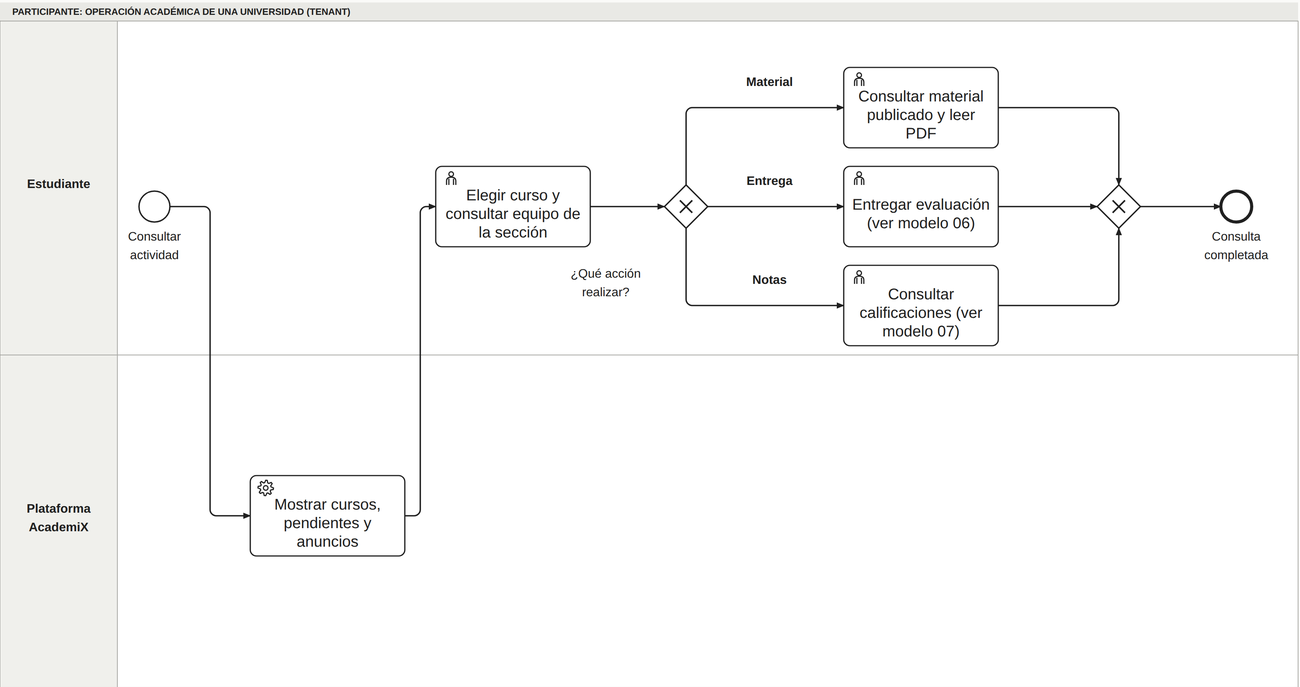
\includegraphics[width=0.31\textwidth]{images/bpmn-05-student-activity.png} &
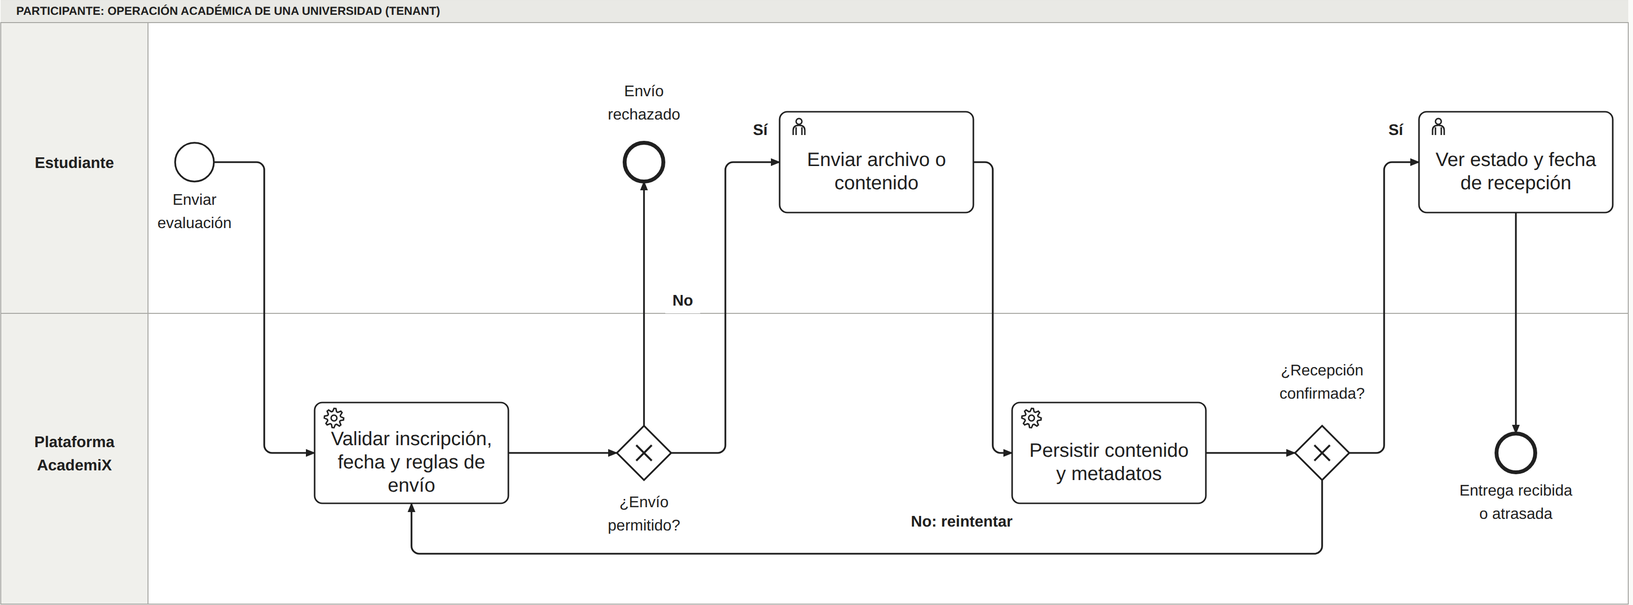
\includegraphics[width=0.31\textwidth]{images/bpmn-06-student-delivery.png} &
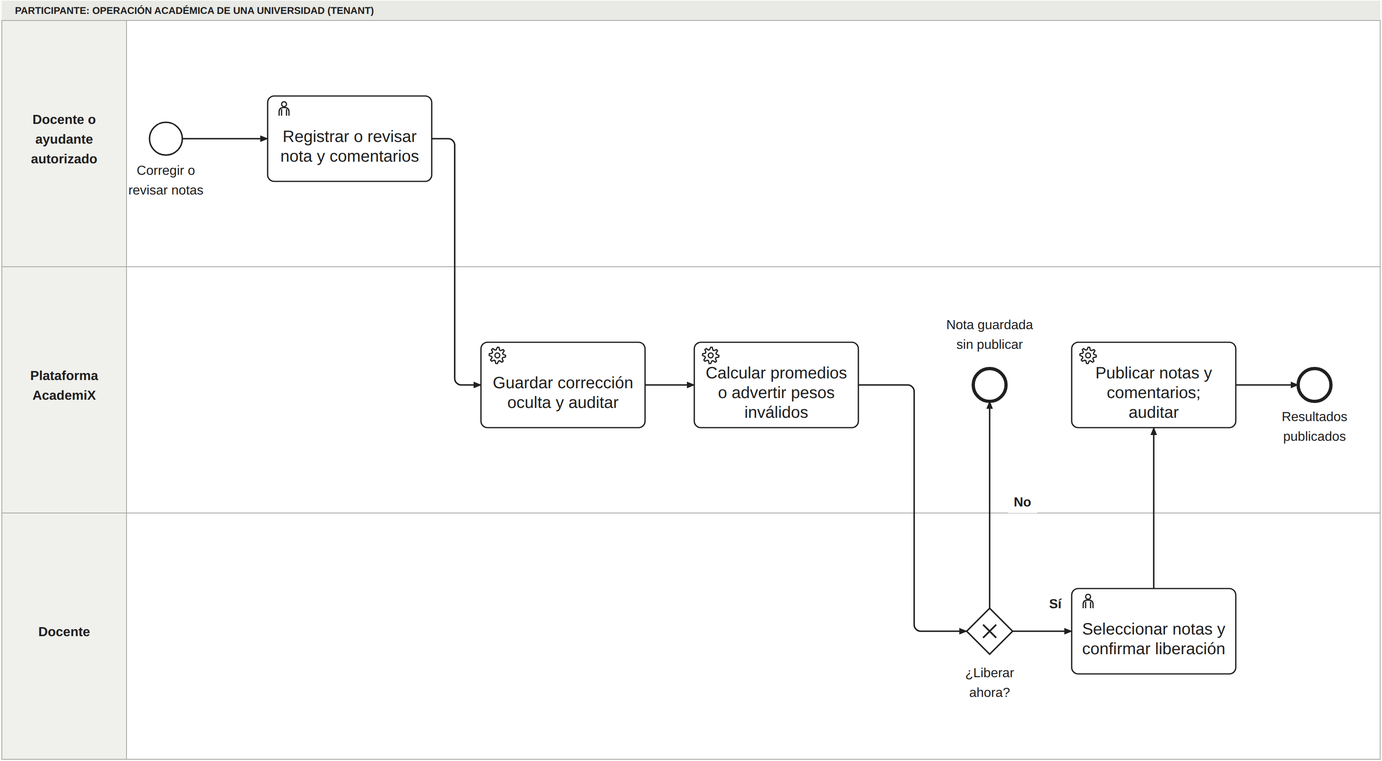
\includegraphics[width=0.31\textwidth]{images/bpmn-03-teaching-correction-publication.png} \\
\footnotesize Actividad del estudiante & \footnotesize Entrega del estudiante & \footnotesize Corrección y publicación \\
\end{tabular}\\
\tightcaption{Figura 1. Modelos de Proceso: consulta de cursos, material y calificaciones; validación y recepción de entregas con posibilidad de reintento; y registro de correcciones, cálculo de promedios y liberación explícita de notas.}
\end{center}


\section{4. Riesgos}

{\small
\setlength{\LTpre}{0pt}
\setlength{\LTpost}{3pt}
\begin{longtable}{|p{1.55cm}|p{2.9cm}|*{2}{>{\raggedright\arraybackslash}p{\dimexpr(\textwidth-1.55cm-2.9cm-8\tabcolsep-5\arrayrulewidth)/2\relax}|}}
\hline
\textbf{Tipo} & \textbf{Riesgo} & \textbf{Impacto} & \textbf{Mitigación} \\
\hline
\endhead
Desarrollo & Sobrealcance funcional & No llegar a un MVP demostrable al cierre del semestre. & Fundaciones primero; las extensiones \emph{nice to have} sólo se activan una vez validadas. \\
\hline
Desarrollo & Complejidad de multi-tenancy & Errores de aislamiento de datos o de permisos. & Registry central, estructura de datos idéntica en cada tenant y pruebas explícitas de acceso cruzado. \\
\hline
Desarrollo & Grupos de estudiantes & Cambiar el modelo de entregas a mitad de camino. & Mantener entregas individuales hasta especificar membresías, permisos y autoría grupal. \\
\hline
Desarrollo & Carga en ventanas críticas & Fallas justo en cierres de entrega y publicación de notas. & Primero consultas eficientes y backend stateless replicable; balanceo, pool, caché y workers entran cuando el plan técnico los justifique. \\
\hline
Desarrollo & Crecimiento de archivos & Saturación de la base de datos y costo de almacenamiento. & Binarios en object storage; en la base sólo metadatos y referencias. \\
\hline
Negocio & Agotamiento del crédito cloud & Perder el ambiente público antes del cierre del proyecto. & Crédito acotado al periodo del proyecto, servicios administrados con escala a cero y límites declarados como supuesto. \\
\hline
Negocio & Competencia con LMS establecidos & Diferencial poco claro frente a Canvas o Moodle. & Competir por integración del flujo crítico y transparencia de calificaciones, no por cantidad de funcionalidades. \\
\hline
Negocio & Baja adopción del flujo & El equipo docente y los estudiantes vuelven a planillas y carpetas externas. & Cada vista nace de una historia con criterios de aceptación y se valida en maquetas antes de programar. \\
\hline
Negocio & IA prematura & Costo variable y distracción del core académico. & Mantener la IA posterior al core, acotada a material publicado o al documento abierto, con citas verificables. \\
\hline
\end{longtable}}

\section{5. Detalle de la solución propuesta}

\textbf{Requisitos funcionales, trazabilidad y beneficio.} El alcance se ordena por bloques; cada bloque referencia requisitos e historias con su prioridad MoSCoW. Los RFO son requisitos funcionales opcionales para las funcionalidades \emph{nice to have}, condicionados al avance.

{\small
\begin{tabularx}{\textwidth}{|p{2.5cm}|p{2.05cm}|Y|Y|}
\hline
\textbf{Bloque} & \textbf{RF} & \textbf{Historias (prioridad)} & \textbf{Beneficio para cliente y usuario} \\
\hline
Tenant, permisos y cuerpo docente & RF1--RF5, RF21 & US5--US7, US30 (must), US8 (should) & Cada universidad opera aislada, los roles se asignan por tenant y por curso, y el estudiante identifica a su equipo docente. \\
\hline
Contenido del curso & RF6--RF8 & US9, US11 (must), US10, US12 (should) & El material queda vinculado al curso y visible sólo cuando el docente publica. \\
\hline
Evaluaciones y entregas & RF9--RF12 & US13--US15 (must), US16 (should) & Fecha, puntaje y evidencia de envío con estado explícito para ambos lados. \\
\hline
Cálculo, corrección y notas & RF13--RF16, RF19, RF22 & US17--US20 (must), US21 (should) & Promedios calculados según ponderaciones, comentarios registrados y publicación manual; el estudiante sabe cuándo su promedio es parcial. \\
\hline
Dashboard y anuncios & RF18 & US1, US2 (must), US3, US4, US23, US24 (should) & Vista única de pendientes y comunicación del curso. \\
\hline
Extensiones del core & RF20 (should), RF17, RFO5 (could) & US26 (should), US22, US25 (could) & Lector de PDF en plataforma; recorrección y calendario interno si el avance lo permite. \\
\hline
Extensiones \emph{nice to have} & RFO1--RFO4, RFO6 (could), RFO7 (fuera) & US27--US29, US31--US36 (could), US37 (fuera) & Video, resumen mediante IA, chats y alertas internas; las alertas por correo quedan como evolución posterior. \\
\hline
\end{tabularx}}

Los RF1 (autenticación), RF6 (configuración general del curso) y RF19 (registro de cambios) son habilitadores transversales para otros requerimientos y por lo tanto no cuentan con historia propia. Se validan a través de las historias de los bloques que los usan.

\textbf{Restricciones.} (i) Ventana efectiva estimada de 10 a 12 semanas dentro de un semestre académico. (ii) Despliegue público con costo controlado. (iii) MVP acotado al core académico. (iv) Google Calendar, Outlook y quizzes en vivo quedan fuera del primer MVP. (v) La IA queda como extensión experimental posterior al core. (vi) El modelo inicial considera entregas individuales: grupos, chats grupales y entregas grupales exigen especificación previa. (vii) Las extensiones \emph{nice to have} sólo se activan después de validar las fundaciones.

\textbf{Requisitos no funcionales como atributos de calidad.} Cada RNF se declara con la acción de diseño que lo sostiene y la evidencia con que se verificará. En lugar de metas numéricas prematuras, se fijan escenarios de calidad que describen la reacción esperada frente a fallas probables.

{\small
\setlength{\LTpre}{0pt}
\setlength{\LTpost}{3pt}
\begin{longtable}{|p{2.45cm}|*{2}{>{\raggedright\arraybackslash}p{\dimexpr(\textwidth-2.45cm-6\tabcolsep-4\arrayrulewidth)/2\relax}|}}
\hline
\textbf{Atributo (RNF)} & \textbf{Acción de diseño / mitigación} & \textbf{Evidencia verificable} \\
\hline
\endhead
Aislamiento y seguridad (RNF3, RNF4) & Tenant resuelto en cada request contra un registry central; base de datos por tenant; autorización por TenantMembership y CourseMembership. & Escenario de acceso cruzado: la operación se bloquea cuando tenant, curso o sección no coinciden, con pruebas automatizadas. \\
\hline
Auditabilidad (RNF5) & Registrar actor, fecha, acción, valor anterior y valor nuevo en cambios de notas, ponderaciones, entregas y liberaciones. & Reconstruir el historial completo de una nota desde la auditoría. \\
\hline
Integridad de la evidencia académica & Confirmar la recepción de una entrega sólo cuando archivo y metadatos quedan persistidos; ante falla, error recuperable y reintento. & Prueba de subida fallida que no deja entrega ni nota inválida. \\
\hline
Disponibilidad (RNF1) & Despliegue reproducible en servicios administrados, logs de error y capacidad de reinicio o redespliegue; balanceo cuando existan varias réplicas. & Escenario de caída parcial de instancia y monitoreo durante las ventanas críticas del semestre. \\
\hline
Rendimiento (RNF6) & Respuesta estable en carga normal y degradación controlada en ventanas críticas: optimizar consultas, acotar bloques secundarios, agregar índices y medir endpoints \emph{antes} de introducir caché. & Medición de los endpoints de dashboard y curso como condición previa a habilitar caché. \\
\hline
Escalabilidad (RNF2) & Frontend y backend stateless replicables; el tenant es el shard desde el inicio; réplica de lectura por tenant cuando ese tenant la justifique. & Supuesto de carga documentado (\emph{spike} cercano a 1.000 concurrentes) usado como caso de diseño del flujo de entrega. \\
\hline
Persistencia de archivos (RNF8) & Binarios en object storage; en PostgreSQL sólo metadatos y \texttt{storage\_key}. & Recursos y entregas recuperables desde el object storage con su metadato. \\
\hline
Recuperabilidad y observabilidad (RNF9, RNF10) & Backup y restore por tenant; logs y métricas básicas de error y carga. & Restore de un tenant sin afectar a los demás; trazas disponibles ante error operacional. \\
\hline
Mantenibilidad (RNF7) & Monolito modular por dominio antes de considerar microservicios. & Módulos separados por dominio y decisiones registradas como ADR. \\
\hline
\end{longtable}}

\textbf{Tecnologías y justificación.} \st{Stack:} Next.js como cliente web que consume la API (vistas por rol, dashboard y curso), NestJS como monolito modular con límites de dominio explícitos, PostgreSQL para los datos académicos transaccionales (notas, ponderaciones y estados exigen restricciones y transacciones) y Docker para un entorno reproducible entre integrantes. \st{Proveedor:} Google Cloud Platform, por su crédito gratuito de USD 300 por tres meses, que cubre el desarrollo y la demo final: Cloud Run para frontend y backend como contenedores stateless, Cloud SQL para las bases por tenant y el registry, Cloud Storage para binarios y Cloud Load Balancing cuando se requiera. Esta elección permite a la arquitectura no estar ligada a un proveedor y en principio los componentes se pueden portar de un proveedor a otro. \st{Condicional:} balanceador o API gateway al desplegar más de una réplica, y pool de conexiones (PgBouncer) cuando la cantidad de tenants o la concurrencia presione los límites de conexiones. \st{En veremos:} Redis y workers entran juntos --- Redis es la cola de los workers --- sólo al implementar las historias que los justifiquen: procesamiento de archivos (US11, US14), recálculo de promedios al cambiar ponderaciones (US17) y despacho de notificaciones (US35, RFO6). Hasta entonces el procesamiento es sincrónico.

\begin{center}
\resizebox{0.93\textwidth}{!}{%
\begin{tikzpicture}[
  font=\sffamily\footnotesize,
  base/.style={draw=navy,thick,fill=soft,rounded corners=2pt,align=center,inner sep=3pt,text width=2.6cm},
  cond/.style={draw=amber,thick,dashed,fill=white,rounded corners=2pt,align=center,inner sep=3pt,text width=2.6cm},
  maybe/.style={draw=slate,thick,dotted,fill=white,rounded corners=2pt,align=center,inner sep=3pt,text width=2.6cm},
  fl/.style={-{Latex[length=1.8mm]},draw=navy,thick},
  fld/.style={-{Latex[length=1.8mm]},draw=amber,thick,dashed},
  flm/.style={-{Latex[length=1.8mm]},draw=slate,thick,dotted},
]
\node[base] (u) at (0,0) {\textbf{Usuarios}\\estudiante · docente\\ayudante · admin};
\node[base] (fe) at (3.6,0) {\textbf{Next.js}\\frontend web\\Cloud Run};
\node[base,text width=3.2cm] (be) at (7.5,0) {\textbf{NestJS modular}\\Cloud Run\\Auth JWT · Tenant Resolver};
\node[cond] (lb) at (5.55,1.9) {\textbf{Load balancer}\\API gateway};
\node[base] (treg) at (11.6,1.9) {\textbf{Tenant Registry}\\PostgreSQL central\\subdominio $\rightarrow$ config};
\node[cond] (cp) at (11.6,0) {\textbf{Connection pool}\\PgBouncer};
\node[base,text width=3.0cm] (db) at (15.4,0) {\textbf{PostgreSQL por tenant}\\Cloud SQL\\1 shard = 1 tenant};
\node[base] (gcs) at (11.6,-1.9) {\textbf{Cloud Storage}\\material y entregas};
\node[maybe] (redis) at (11.6,-3.6) {\textbf{Redis}\\cola y caché};
\node[maybe] (wk) at (15.4,-3.6) {\textbf{Workers}\\fuera del request};
\draw[fl] (u) -- (fe);
\draw[fl] (fe) -- (be);
\draw[fld] (fe) |- (lb);
\draw[fld] (lb) -| (be);
\draw[fl] (be) |- (treg);
\draw[fld] (be) -- (cp);
\draw[fl] (cp) -- (db);
\draw[fl] (be) |- (gcs);
\draw[flm] (be) |- (redis);
\draw[flm] (redis) -- (wk);
\node[align=left,font=\sffamily\scriptsize] at (3.4,-3.6) {%
\textcolor{navy}{\textbf{---}}~base, desde el primer despliegue\\
\textcolor{amber}{\textbf{-- --}}~condicional, al desplegar o con carga\\
\textcolor{slate}{\textbf{$\cdots$}}~en veremos, atado a una historia};
\end{tikzpicture}}\\
\tightcaption{Figura 2. Arquitectura candidata. La ruta base es cliente, frontend, backend modular, registry, base por tenant y object storage; el resto está diseñado pero no comprometido para el primer despliegue.}
\end{center}

\textbf{Primeras maquetas.} Las maquetas son wireframes navegables en HTML estático; cada vista declara las historias que valida y no tiene backend.

\begin{center}
\begin{tabular}{ccc}
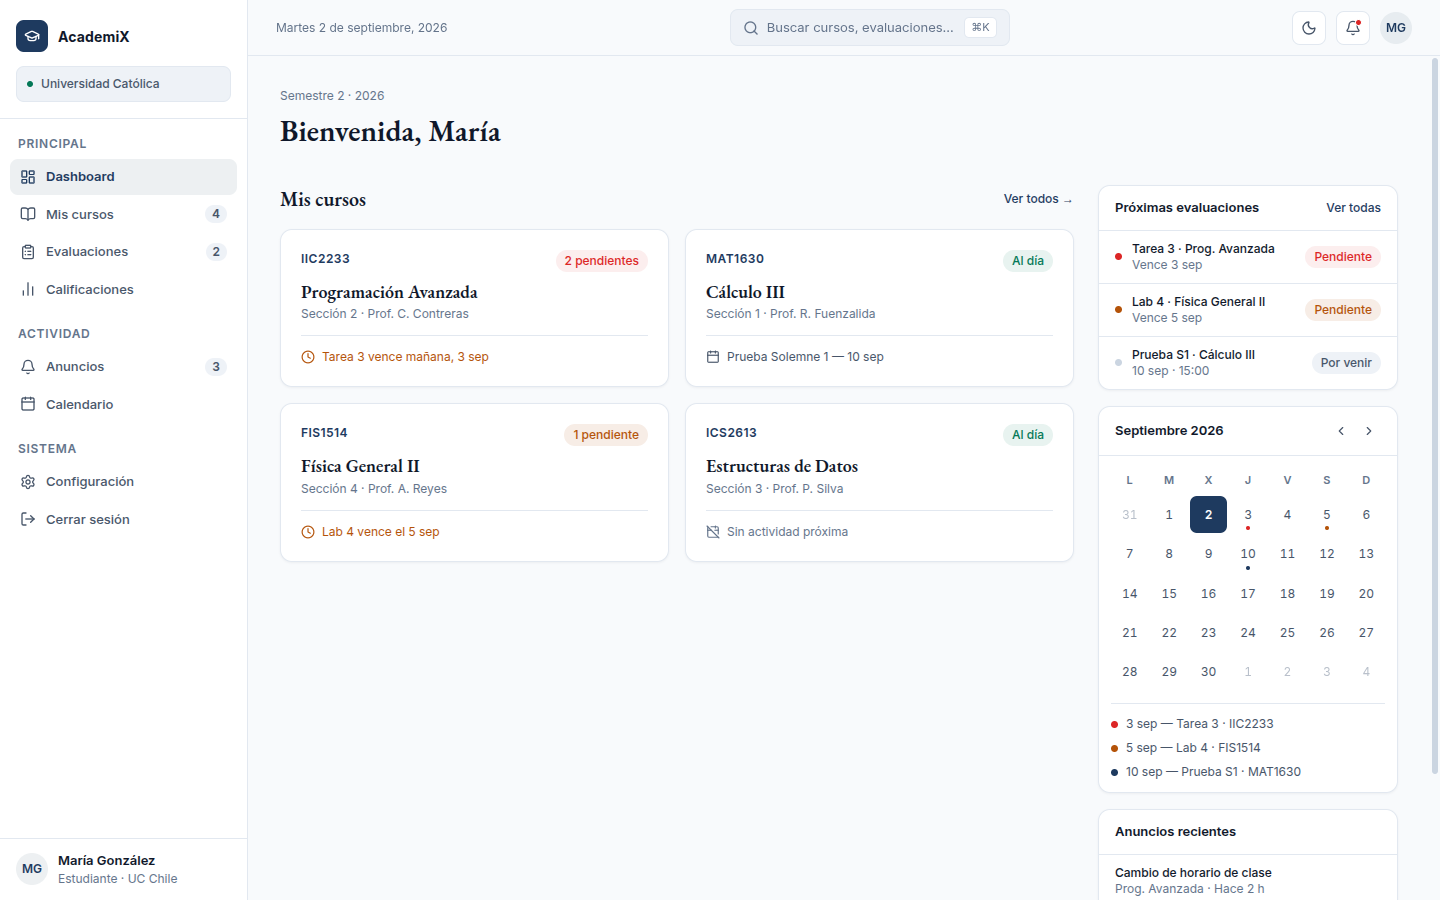
\includegraphics[width=0.31\textwidth]{images/mockup-dashboard.png} &
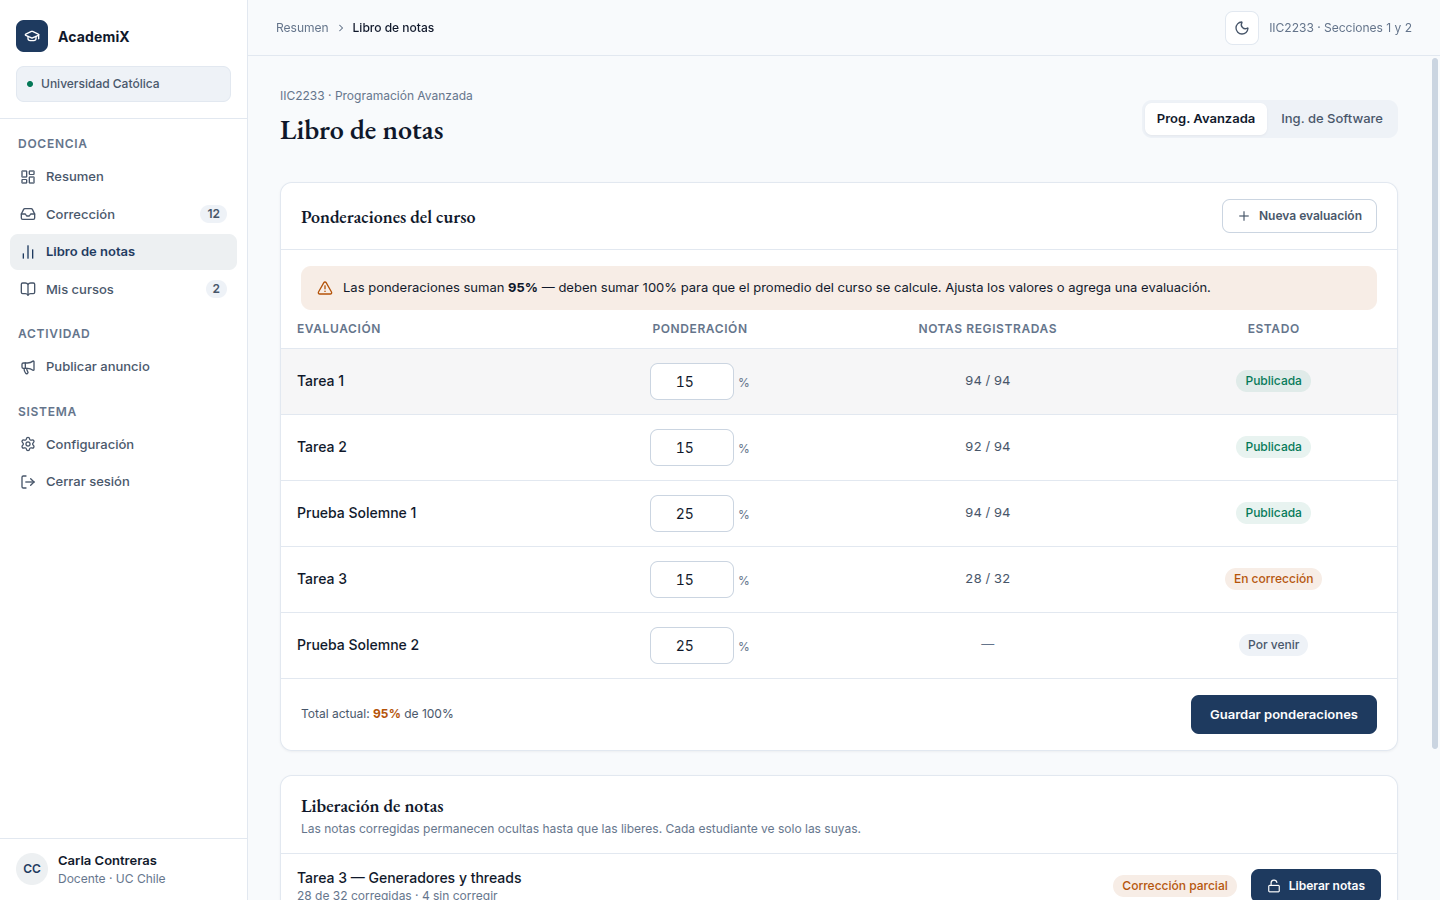
\includegraphics[width=0.31\textwidth]{images/mockup-teacher-gradebook.png} &
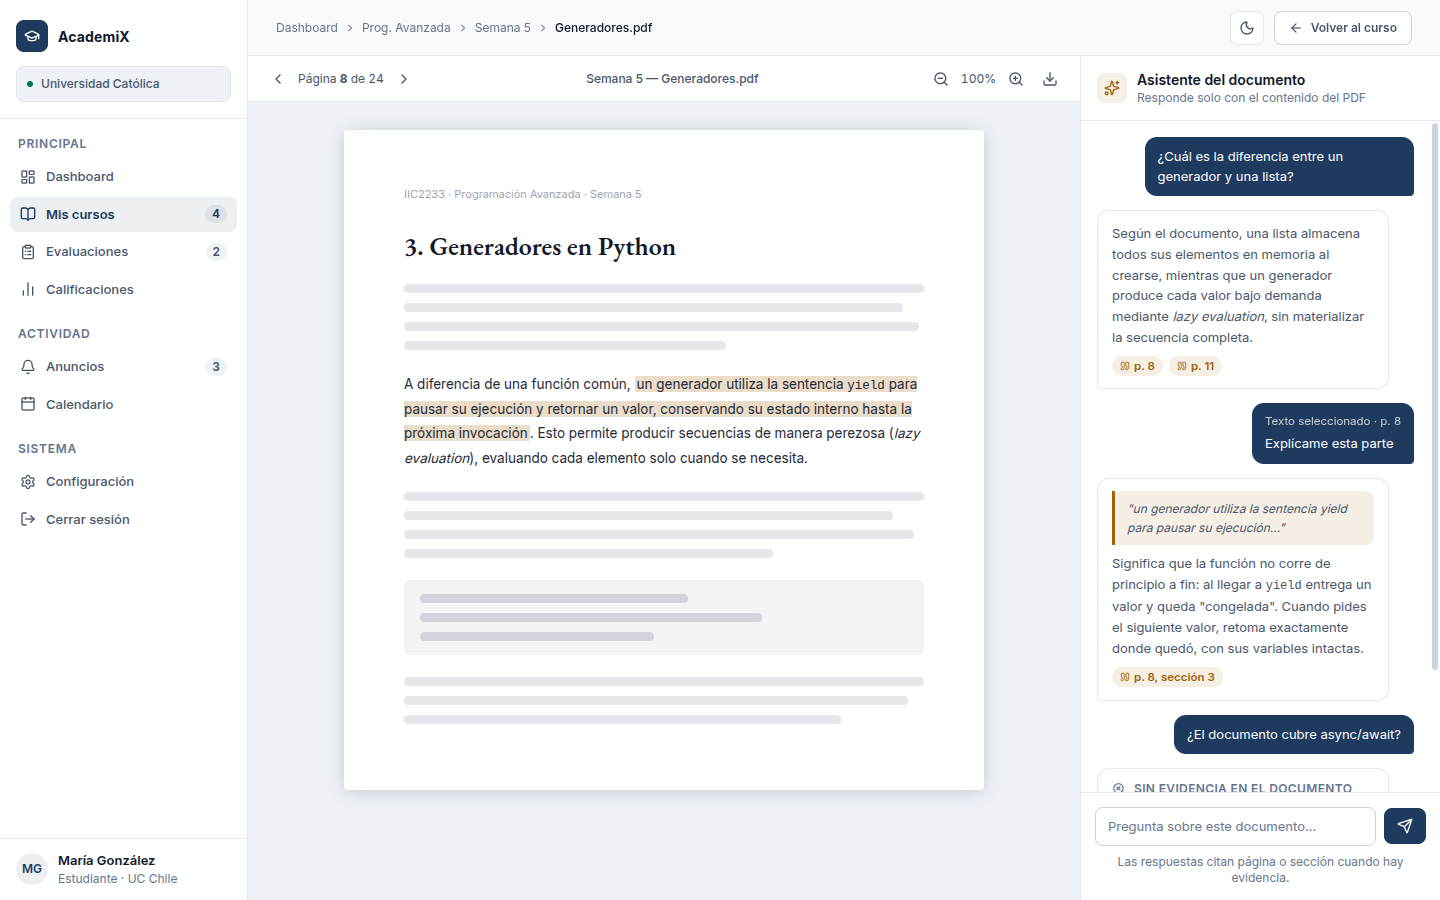
\includegraphics[width=0.31\textwidth]{images/mockup-pdf-reader.png} \\
\footnotesize Dashboard estudiante (US1--US3) & \footnotesize Libro de notas docente (US17, US18) & \footnotesize Lector PDF e IA (US26--US29) \\
\end{tabular}\\
\tightcaption{Figura 3. Maquetas de referencia: core del estudiante, control docente de calificaciones y extensión condicionada.}
\end{center}

\textbf{Decisiones abiertas.} Se declaran para no presentar como cerrado lo que aún no está decidido:
\begin{itemize}
  \item \textbf{Umbrales de rendimiento.} No se comprometen cifras: se fijan midiendo los endpoints de dashboard y curso, y esa medición decide si entra caché.
  \item \textbf{Activación de Redis y workers.} Se resuelve al especificar la historia que los justifique; hasta entonces el procesamiento es sincrónico.
  \item \textbf{Modelo de grupos de estudiantes.} Habilitar chat de grupo o entregas grupales exige definir grupos, membresías y autoría; sin eso, el modelo se mantiene individual.
  \item \textbf{Extensiones \emph{nice to have} que entran.} Depende del avance real al cerrar las fundaciones; no se compromete el conjunto completo.
  \item \textbf{Modelo y costo del asistente de IA.} Sin definir, coherente con dejarlo posterior al core.
\end{itemize}

\section{6. Plan de trabajo}

El roadmap enumera 12 iteraciones semanales dentro de una ventana efectiva de 10 a 12 semanas; las iteraciones 11 y 12 operan como colchón de cierre y pueden comprimirse.

{\small
\begin{tabularx}{\textwidth}{|p{1.1cm}|Y|p{3.2cm}|Y|}
\hline
\textbf{Sem.} & \textbf{Actividades técnicas (RF/RNF)} & \textbf{Actividades no técnicas} & \textbf{Que se espera completar} \\
\hline
1--2 & Setup del monorepo, base Next.js y NestJS, autenticación y resolución de tenant (RF1, RF2, RNF3, RNF4). & Visión, modelo de dominio, arquitectura, maquetas y backlog priorizado. & Usuario autenticado y tenant resuelto en cada request. \\
\hline
3--4 & Periodos, cursos, secciones, inscripciones, cuerpo docente visible, módulos, material y object storage (RF3--RF8, RF20, RF21, RNF8). & Validación de maquetas de curso y refinamiento del backlog. & Un curso real con secciones, participantes y material publicado. \\
\hline
5--7 & Evaluaciones y pendientes, entregas, corrección, comentarios y liberación manual (RF9--RF13, RF16). & Criterios de aceptación por historia y revisión cruzada entre pares. & Ciclo evaluación--entrega--corrección sin publicación automática. \\
\hline
8--9 & Libro de notas, cálculo de promedios, auditoría, dashboard y anuncios (RF14, RF15, RF18, RF19, RF22, RNF5). & Demo intermedia y decisión de qué extensiones se activan. & Docente y estudiante ven la misma verdad sobre calificaciones. \\
\hline
10--11 & Despliegue público, observabilidad, decisiones de rendimiento, hardening de permisos y pruebas de flujos críticos (RNF1--RNF4, RNF6, RNF9, RNF10). & Coordinación de infraestructura y ADR de las decisiones abiertas. & Ambiente público operativo con permisos verificados. \\
\hline
12 & Cierre de deuda crítica y ajustes finales de UX. & Demo final, documentación y presentación. & Entrega final demostrable y caso de negocio validado. \\
\hline
\end{tabularx}}

\section{7. Glosario y anexos}

{\small
\begin{multicols}{2}
\textbf{Tenant:} universidad aislada dentro de la plataforma.\\
\textbf{Tenant registry:} base central que resuelve el subdominio a la configuración del tenant.\\
\textbf{Shard:} partición de datos; aquí un shard equivale a un tenant desde el inicio.\\
\textbf{Curso:} ramo semestral concreto de un periodo académico.\\
\textbf{Sección:} grupo de estudiantes dentro de un curso.\\
\textbf{Módulo:} bloque de contenido; semana, tema o unidad.\\
\textbf{Recurso:} material publicado en un módulo (PDF, PPT, enlace).\\
\textbf{Evaluación:} actividad con entrega, corrección, nota y ponderación.\\
\textbf{Entrega:} envío de un estudiante para una evaluación.\\
\textbf{Liberación de notas:} acción del docente que hace visible una nota.\\
\textbf{Libro de notas:} vista consolidada de evaluaciones, ponderaciones y promedio.\\
\textbf{Recorrección:} solicitud de revisión de una calificación publicada.\\
\textbf{Rol contextual:} rol que depende del tenant y del curso, no del usuario global.\\
\textbf{Escenario de calidad:} falla probable descrita junto a la reacción esperada del sistema.\\
\textbf{Object storage:} almacenamiento de binarios fuera de la base relacional.\\
\textbf{RFO:} requisito funcional opcional, condicionado al avance del proyecto.
\end{multicols}}

\textbf{Anexo A. Trazabilidad RF $\rightarrow$ historias de usuario.} RF1: habilitador. RF2: US5, US8, US12, US30. RF3: US5. RF4: US5, US6. RF5: US7, US8. RF6: habilitador. RF7: US9, US10. RF8: US11, US12. RF9: US13, US17. RF10: US2, US16. RF11: US14. RF12: US15. RF13: US18. RF14: US19, US20. RF15: US17, US19, US20. RF16: US15, US21. RF17: US22. RF18: US1--US4, US23, US24. RF19: habilitador (soporta RNF5). RF20: US26. RF21: US30. RF22: US17, US20. RFO1: US31. RFO2: US32. RFO3: US33. RFO4: US34. RFO5: US25. RFO6: US35, US36. RFO7: US37 (fuera del alcance inicial).


\end{document}
